\section{Constraint Satisfaction Problem }\index{Constraint Satisfaction Problem }
Constraint satisfaction problems(CSP) are mathematical problems defined as a set of objects whose state must satisfy a number of constraints or limitations. One example of a CSP is the game “Sudoku” \\[3ex]

\section{Basic terms about CSP:}
\begin{itemize}
\item an assignment is to assign values to some or all variables
\item an assignment that does not violate any constraints is called a consistent assignment. With values from domain D\_i
\item A complete assignment is one in which each variable is assigned
\item a partial assignment is one that assigns value to some of the variables 
\end{itemize}


\textbf{Constraint graph}\\
Binary CSP: each constraint relates at most two variables, e.g: WASA
constraint graph: nodes are variables(e.g. region WA), arcs show constraints(e.g. WASA)\\[3ex]

\textbf{Varieties of Variables}\\
Discrete variables
\begin{itemize}
\item Finite Domains
\item boolean CSPs, include: boolean satisfiability(NP - complete)
\item Sudoku
\item Infinite Domains(Integers, Strings, etc.)

\item job scheduling, variables are start/end days for each job, need a constraint language, e.g. $StartJob_1$ + 5 $\leq  StarJob_3$
\end{itemize}
Continuous variables
\begin{itemize}
\item start /end times for Hubble Telescope observations
\item Unary constraints involve a single variable
\setlength{\itemindent}{3em}
\item $SA \neq Green$
\setlength{\itemindent}{0em}
\item binary constraints involve pairs of variables
\setlength{\itemindent}{3em}
\item $SA \neq WA$
\setlength{\itemindent}{0em}
\item Higher-order constraints involve 3 or more variables	
\setlength{\itemindent}{3em}
\item cryptarithmetic column constraints
\setlength{\itemindent}{0em}
\item Preferences(soft) constraints
\setlength{\itemindent}{3em}
\item red  is better than green
\item CSPs with preference are often with optimization search algorithms constraints optimization problems 
\end{itemize}


\subsection{Node Consistency}
If a node is node-consistent if all the value’s domain satisfy the variable’s unary constraints.\\[3ex]

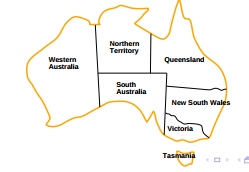
\includegraphics[scale=1]{chap1_pics/austaliaareas.png} 

Example:\\
D = {Red, Green, Blue}\\
Variable X\\
X dislikes green, then X starts with D = {Red, Green, Blue}, and becomes node consistent after eliminating {Green}.
X is node consistent with the reduced domain, D={Red, Blue}.\\

\textbf{Arc Consistency}\\
$X_i$ is arc-consistent with respect to another variables $X_j$ if for every value in $X_i$’s current domain $D_i$ there is one value in $X_i$’s domain $D_j$ that satisfies the binary constraint on the arc $(X_i , X_j)$\\[3ex]

Example:\\
Given two variables $X_i$ , $X_j$ with values in {0,1,2,...9} and constraints 
(0,0),(1,1),(2,4),(3,9).\\
To make $X_i$ arc-consistent with respect to $X_j$, we reduce $X_i$’s domain to {0,1,2,3}.\\
To make $X_j$ arc-consistent with respect to $X_i$, we reduce $X_j$’s domain to {0,1,4,9}.\\

\section{Arc Consistency Algorithm(AC-3)}
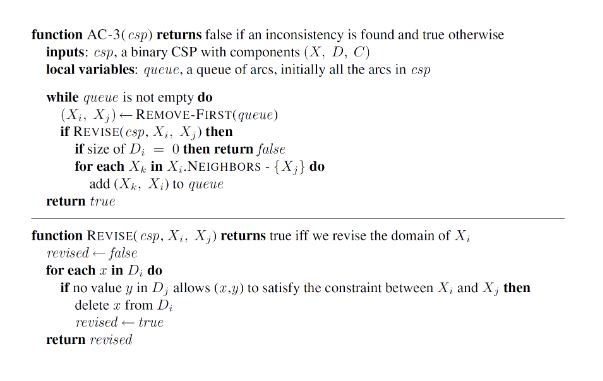
\includegraphics[scale=1]{chap1_pics/1nAyMlelLl-LW-ECO-Akl5AsNAugdRshrNF4o7Q.png} 
\begin{enumerate}
\item initially let a queue contain all arcs
\item remove an arc $(X_i , X_j)$ from the queue and make the variable $X_i$ arc-consistent to $X_j$
\begin{enumerate}
\item IF$ X_i$ domain $D_i$ is unchanged, then check the next arc in the queue
\item IF $X_i$ ‘s domain $D_i$ is revised(smaller), then add all arcs $(X_k, X_i) $in the queue 
\item If $X_i$ ’s domain $D_i$ is empty, then CSP no solution
\end{enumerate}
\item Keep checking all arcs in the queue until the queue is empty 
\end{enumerate}

\section{Path consistency}
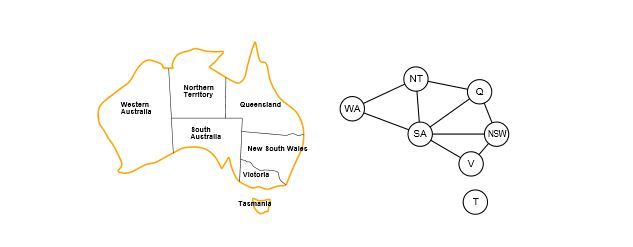
\includegraphics[scale=1]{chap1_pics/patchconsistency.jpeg} 
A two variable set ${X_i,X_j}$ is path consistency with respect to a third variable $X_m$ if for every assignment ${X_i = a, X_j = b}$ consistent with the constraints on${X_i, X_j}$, where is an assignment to $X_m$ ,that satisfies the constraints on${X_i , X_m}$ and ${X_m, X_j}$ \\[3ex]

Example:\\
Can we color the Australia map with two colors?\\
Make the set {WA, SA} path consistent with respect to NT?\\
Assignments: {WA = blue, SA = red} or {WA =blue,SA=red}\\
But no assignment exists for NT\\[3ex]

\textbf{Constraint propagation}
\begin{itemize}
\item constraint propagation is a specific type of inference 
\begin{itemize}
\item use the constraints to reduce the number of legal values for a variable, which in turn can reduce the legal values for another variable, and so on
\end{itemize}

\item node consistency
\item arc consistency
\item path consistency 
\item k-consistency: k variables involved
\item Global consistency 

\end{itemize}

\textbf{Limits}
\begin{itemize}
\item Indeed AC-3 works for the easiest Sudoku puzzles
\item slightly harder ones can be solved by PC-2, but at a greater computational cost: there are 255,960 
different path constraints to consider in a Sudoku puzzle
\item To solve the hardest puzzles and to make efficient progress, we will have to be more clever 

\end{itemize}

\section{Backtracking}
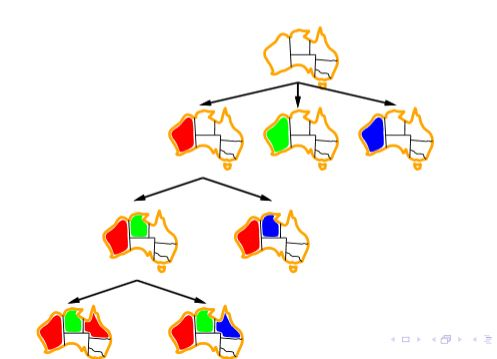
\includegraphics[scale=1]{chap1_pics/backtracking.jpeg} 

\begin{enumerate}
\item Select an unassigned value
\item assign values
\item Depth-first search
\item If an inconsistency is detected, then BACKTRACK returns failure, causing the previous call to try another value
\end{enumerate}

Backtracking search is a depth-first search for CSPs
\begin{itemize}
\item choose values for one variable at a time
\item backtrack when a variables has no legal left to assign
\end{itemize}
Backtracking search is the basic uninformed algorithm for CSP.
Can solve n-queens for $n\approx 25.$

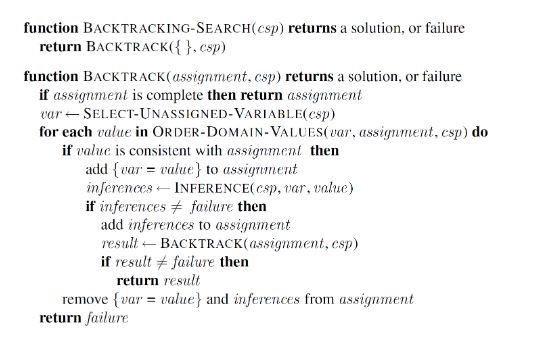
\includegraphics[scale=1]{chap1_pics/backtrackcode.jpeg}
\subsection{Improving backtracking efficiency}
General-purpose methods can give huge gains in speed:\\
\begin{enumerate}
\item which variable should be assigned next?
\item in what order should values be tried`?
\item can we detect inevitable failure early?
\item Can we take advantage of problem structure? 
\end{enumerate}

\textbf{Minimum remaining values}\\
Minimum remaining values (MRV): choose the variable with the fewest legal values.

\textbf{Degree heuristic}\\
\begin{itemize}
\item Tie-breaker among MRV variables
\item Degree heuristic: choose the variable with the most constraints on remaining variables 
\end{itemize}

\includegraphics[scale=1]{chap1_pics/backtrack2.jpeg}

\textbf{Least constraining value}\\
Given a variable, choose the least constraining value: the one that rules out the fewest values in the remaining variables.\\

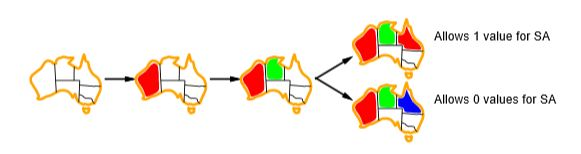
\includegraphics[scale=1]{chap1_pics/backtrack3.jpeg}
Combining these heuristics makes 1000 queens feasible.\\


\subsection{Forward checking}
Idea: Keep track if remaining legal values for unassigned variables.\\
Terminates search when any variable has no legal values.\\

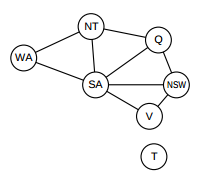
\includegraphics[scale=1]{chap1_pics/australiamap.png}\\
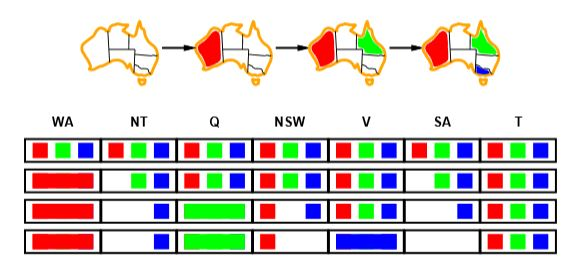
\includegraphics[scale=1]{chap1_pics/backtrack4.jpeg}

\textbf{Constraint propagation}\\
Forward checking propagates information from assigned to unassigned variables, but doesn’t provide early detection for all failures: \\
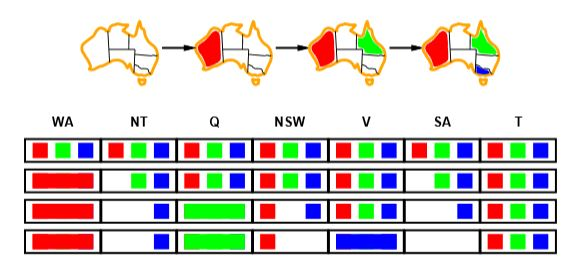
\includegraphics[scale=1]{chap1_pics/backtrack4.jpeg}

NT and SA cannot both be blue!\\
Constraint propagation repeatedly enforces constraints locally.\\

\subsection{Arc consistency}
Simplest form of propagation makes each arc consistent.\\
$X \rightarrow  Y$ is consistent if for every value x of X there is some allowed y \\[3ex]
If X looses a value, neighbours needs to be rechecked.\\
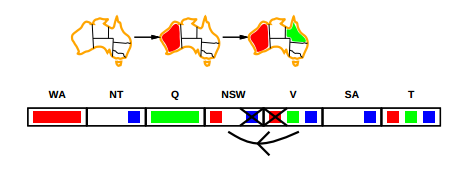
\includegraphics[scale=1]{chap1_pics/arcconsistency1.png} 

Arc consistency detects failure earlier than \textit{forward checking}.
Can be run as a predecessor or after each assignment.

\section{Structure}
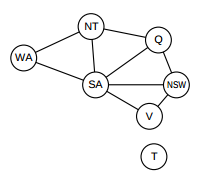
\includegraphics[scale=1]{chap1_pics/australiamap.png}\\
Tasmania and mainland Australia are independent subsections which can be identified as connected components of constraint graph. \\

\begin{itemize}
\item Suppose each subproblem has a \textit{c} variable out of \textit{n} total
\item Worst-case solution cost is $ n/c * d^c$ liniar in \textit{n}
\item E.g. $n = 80, d = 2, c =20$
\begin{itemize}
\item $2^{80}$ = 4 billion years at 10 million nodes/sec
\item $2 * 2^{20} = 0.4$ seconds at 10 million nodes/sec
\end{itemize}
\end{itemize} 

\subsection{Tree-structure CSPs}
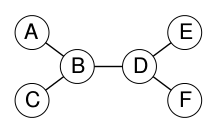
\includegraphics[scale=1]{chap1_pics/treestructure.png}

\begin{itemize}
\item Theorem: if the constraitn graph has no loops, the CSP can be solved in $O(nd^2)$ time
\item Compare to general CSPs, where worst-case time is $O(d^n)$
\item This property also applies to logical and probabilistic reasoning: an important example of the relation between syntactic restrictions and the complexity of reasoning
\end{itemize}

\subsection{Algorithm for tree-structured CSPs}
\begin{enumerate}
\item Choose a variable as root, order variables from root to leaves such that every node's parent precedes it in the ordering
\item For \textit{j} from \textit{n} down to 2, apply \textit{RemoveInconsistent}$(Parent(X_j),x_j)$
\item For \textit{j} from 1 to \textit{n}, assign $X_j$ consistently with $Parent(X_j)$
\end{enumerate}
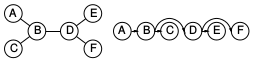
\includegraphics[scale=1]{chap1_pics/treestructurealgorithm.png} 

\subsection{Nearly tree-structured CSPs}
\begin{itemize}
\item Conditioning: instantiate a variable, prune its neighbours domains
\item Cutset conditioning: instantiate(in all ways) a set of variables such that the remaining constraint graph is a tree
\item Cutset size $c \Rightarrow runtime O(d^c * (n-c)d^2)$, very fast for small \textit{c}
\end{itemize}

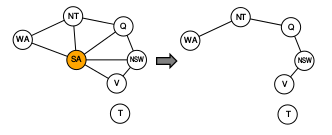
\includegraphics[scale=1]{chap1_pics/treestructuremap.png} 
\label{treestructuremap}

\begin{itemize}
\item Choose a subset \textit{S} from \textit{VARIABLE[csp]} such that the constraint graph becomes a tree after removal of \textit{S}
\item For each possible assignment to the variables in \textit{S} satisfies all constraint on S 
\begin{itemize}
\item remove from the domains of the remaining variables any values that are inconsistent with the assignment of \textit{S}
\item If the remaining CSP has solution, then return it together the assignment to S
\end{itemize}
\end{itemize}

\section{Local Search for CSPs}
\begin{itemize}
\item Local search, e.g. hill-climbing, simulated annealing for CSP
\begin{itemize}
\item typically start with a "complete" state, i.e. all variables assigned to values, but may violated constraints
\item then search changes the value of one variable at each time for violated constraints
\end{itemize}
\item Variable selection: randomly select any conflicted variable
\item Value selection by min-conflicts heuristics:
\begin{itemize}
\item choose value that violates the fewest constraints i.e. hillclimb with $h(n) = $total number of violated constraints
\end{itemize}
\end{itemize}

\subsection{Min-Conflict Algorithms}
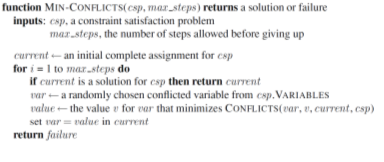
\includegraphics[scale=1]{chap1_pics/minconflictalgoithm.png} 

\begin{itemize}
\item Given random initial state, can solve \textit{n-queens} in almost constant time for arbitrary \textit{n} with high probability (e.g. $n = 10 000 000$)
\item The same to be true for any randomly-generated CSP \textit{except} in a narrow range of the ratio $R=\frac{number of constraints}{number of variables}$
\end{itemize}
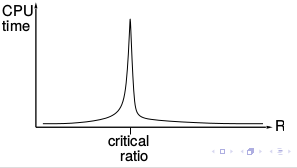
\includegraphics[scale=1]{chap1_pics/minconfliggraph.png} 
